\begin{figure}[!ht]
    \centering

    \begin{subfigure}{0.2\linewidth}
        \centering
        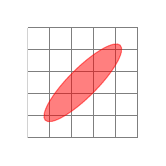
\begin{tikzpicture}[scale=0.7, opacity=0.5]
            \clip (0,0) rectangle (2,2);
            \begin{scope}
                \draw[step=0.4] (0,0) grid (2,2);
            \end{scope}
            \begin{scope}[shift={(1,1)}, rotate=45, xscale=3.7, scale=1.3, shift={(-1,-1)}]
                \draw[color=red, fill=red, fill opacity=0.5] (1,1) circle (0.2);
            \end{scope}
        \end{tikzpicture}
        \caption{}
    \end{subfigure}
    %
    \begin{subfigure}{0.2\linewidth}
        \centering
        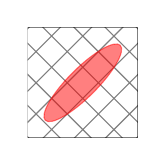
\begin{tikzpicture}[scale=0.7, opacity=0.5]
            \clip (0,0) rectangle (2,2);
            \draw (0,0) rectangle (2,2);
            \begin{scope}[shift={(1,1)}, rotate=45, shift={(-1,-1)}]
                \draw[step=0.4] (-1,-1) grid (3,3);
            \end{scope}
            \begin{scope}[shift={(1,1)}, rotate=45, xscale=3.7, scale=1.3, shift={(-1,-1)}]
                \draw[color=red, fill=red, fill opacity=0.5] (1,1) circle (0.2);
            \end{scope}
        \end{tikzpicture}
        \caption{}
    \end{subfigure}
    %
    \begin{subfigure}{0.2\linewidth}
        \centering
        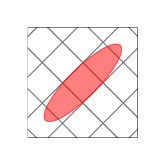
\begin{tikzpicture}[scale=0.7, opacity=0.5]
            \clip (0,0) rectangle (2,2);
            \draw (0,0) rectangle (2,2);
            \begin{scope}[shift={(1,1)}, rotate=45, scale=1.3, shift={(-1,-1)}]
                \draw[step=0.4] (0,0) grid (2,2);
            \end{scope}
            \begin{scope}[shift={(1,1)}, rotate=45, xscale=3.7, scale=1.3, shift={(-1,-1)}]
                \draw[color=red, fill=red, fill opacity=0.5] (1,1) circle (0.2);
            \end{scope}
        \end{tikzpicture}
        \caption{}
    \end{subfigure}
    %
    \begin{subfigure}{0.2\linewidth}
        \centering
        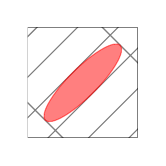
\begin{tikzpicture}[scale=0.7, opacity=0.5]
            \clip (0,0) rectangle (2,2);
            \draw (0,0) rectangle (2,2);
            \begin{scope}[shift={(1,1)}, rotate=45, xscale=3.7, scale=1.3,shift={(-1,-1)}]
                \draw[step=0.4] (0,0) grid (2,2);
            \end{scope}
            \begin{scope}[shift={(1,1)}, rotate=45, xscale=3.7, scale=1.3, shift={(-1,-1)}]
                \draw[color=red, fill=red, fill opacity=0.5] (1,1) circle (0.2);
            \end{scope}
        \end{tikzpicture}
        \caption{}
    \end{subfigure}

    \caption{The original surface mapping (a) is transformed into an anisotropy compensating mapping (d) by rotation (b), isotropic scaling (c), and anisotropic scaling (d) obtained from the pixel filter (red). \label{fig:dimensions}}
\end{figure}